\section{Auswertung}
\label{sec:Auswertung}

\subsection{Fehler}
Für die Auswertung wird die \texttt{Python}-Bibliothek \texttt{numpy} \cite{numpy} benutzt. Die Fits entstehen mit \texttt{curve\_fit} aus \texttt{scipy.optimize} \cite{scipy}.
Die Fehlerrechnung wird mit \texttt{uncertainties} \cite{uncertainties} durchgeführt. Plots entstehen mit \texttt{matplotlib.pyplot} \cite{matplotlib}. \\
Der Mittelwert $\bar{x}$ von $N$ gemessenen Werten $a$ bestimmt sich über
\begin{equation}
    \bar{x} = \frac{1}{N} \sum^N_{i=1} a_i,
    \label{eq:mittelwerte}
\end{equation}
der Fehler des Mittelwertes über
\begin{equation}
    \Delta x = \sqrt{\frac{1}{N \cdot (N-1)} \sum^N_{i=1}(a_i - \bar{x})}.
    \label{eq:mittelwerte_fehler}
\end{equation}
Die Gaußsche Fehlerfortpflanzung für eine berechnete Größe $f$ lautet
\begin{equation}
    \Delta f = \sqrt{ \sum^N_{i=1} \left( \frac{\delta f}{\delta x_i}\right)^2 \cdot (\Delta x_i)^2}.
\end{equation}
Prozentuale Abweichungen werden mit
\begin{equation}
    \Delta x = \left|\frac{x - a}{a}\right|
    \label{eq:abweichung}
\end{equation}
berechnet, wobei $a$ ein Vergleichswert und $x$ der erhaltene Wert ist.
\newpage

\subsection{Magnetfeldstärke}
Im ersten Schritt wird die Stärke des Magnetfelds in Abhängigkeit von der Sondenposition 
gemessen. Das Magnetfeld wird von einem Elektromagneten erzeugt. Die gemessenen Werte sind in \autoref{tab:magnetfeld} angegeben, in Abbildung \ref{fig:magnetfeld} ist die magnetische Flussdichte gegen die Position der Sonde geplottet.

\begin{table}[H]
    \centering
    \caption{Messwerte des Magnetfeldes $B$ bei verschiedenen Positionen $z$.}
    \label{tab:magnetfeld}
    \begin{tabular}{c c}
        \toprule
        {$z$ in $\si{\milli\meter}$} & {$B$ in $\si{\milli\tesla}$} \\
        \midrule
        40  & \num{0.60(5)} \\ 
        50  & \num{1.10(5)} \\ 
        60  & \num{0.80(5)} \\ 
        70  & \num{0.30(5)} \\ 
        80  & \num{0.30(5)} \\ 
        90  & \num{0.30(5)} \\
        100 & \num{0.60(5)} \\ 
        105 & \num{0.90(5)} \\
        110 & \num{1.70(5)} \\ 
        115 & \num{5.00(5)} \\
        120 & \num{17.3(5)} \\ 
        125 & \num{56.9(5)} \\ 
        130 & \num{214.0(5)} \\
        135 & \num{394.0(5)} \\
        140 & \num{421.0(5)} \\ 
        145 & \num{414.0(5)} \\
        150 & \num{354.0(5)} \\ 
        55  & \num{134.0(5)} \\ 
        160 & \num{26.0(5)} \\
        165 & \num{6.0(5)} \\ 
        170 & \num{1.60(5)} \\
        \bottomrule
    \end{tabular}
\end{table}

<<<<<<< HEAD


\begin{figure}[H]
||||||| 05b9994


\begin{figure}
=======
\begin{figure}[H]
>>>>>>> 488e4e5413ead7ea746f355c1424b3fbb286a0b0
    \centering
    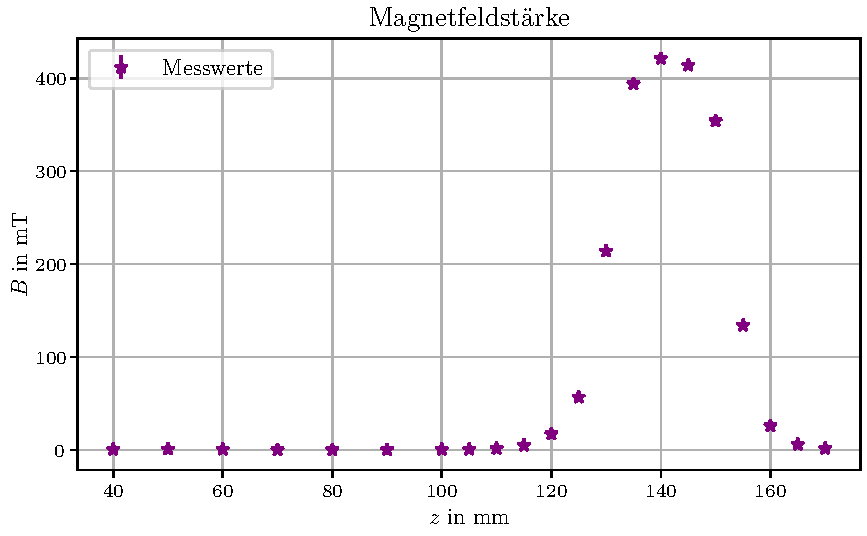
\includegraphics[width=0.8\textwidth]{plots/magnetfeld.pdf}
    \caption{Die Kraftflussdichte $B$ in $\si{\milli\tesla}$ über den Ort $z$ in $\si{\milli\meter}$ in der Spule.}
    \label{fig:magnetfeld}
\end{figure}
Die maximal gemessene Kraftflussdichte beträgt
\begin{equation*}
    B_\text{max} = \qty{421.0(5)}{\milli\tesla}.
\end{equation*}

<<<<<<< HEAD
%%%%%%%%%%%%%
%%%%%%%%%%%%%
% HIER NOCH DIE FEHLER UNTEN ÄNDERN!!!!!!!!!!
%%%%%%%%%%%%%
%%%%%%%%%%%%

||||||| 05b9994
=======

>>>>>>> 488e4e5413ead7ea746f355c1424b3fbb286a0b0
\subsection{Drehwinkel der Faraday-Rotation}
<<<<<<< HEAD
Die folgenden drei Tabellen beinhalten die Wellenlänge des benutzten Lichtes, die gemessenen Winkel sowie die Länge normierten Winkel $\theta_\text{frei}$ nach \autoref{eq:theta} und \autoref{eq:thetafrei}, sowie die Wellenlänge. Die Dotierung und die Dicke der Probe werden jeweils angegeben.
||||||| 05b9994
Der gesamte Drehwinkel, um den rotiert wird, lautet in $\si{\radian}$
\begin{equation*}
    \theta_\text{frei} = \frac{\theta_1-\theta_2}{2} \cdot \frac{\pi}{\qty{180}{\degree}},
\end{equation*} 
wobie $\theta_1$ und $\theta_2$ die vermessenen Winkel für die beiden Polungen des Magnetfeldes in $\si{\degree}$ sind.\\
Die folgenden drei Tabellen beinhalten die gemessenen Winkel, die normierten Winkel, sowie die Wellenlänge. Die Dotierung und die Dicke der Probe werden jeweils angegeben.
=======

Die folgenden drei Tabellen beinhalten die gemessenen Winkel, die normierten Winkel, sowie die Wellenlänge. Die Dotierung und die Dicke der Probe werden jeweils angegeben.
>>>>>>> 488e4e5413ead7ea746f355c1424b3fbb286a0b0
Der Fehler in der Messung für $\theta_{1,2}$ beträgt ca. $\Delta \theta_{1,2} = \qty{0.005}{\degree}$ und die Fehlerfortpflanzung zu $\theta_\text{frei}$ gibt $\Delta \theta = \qty{0.00006}{\radian}$.
Die Wellenlänge ist ohne Fehler auf den Filtern angegeben.

\begin{table}[H]
    \centering
    \caption{Gemessene Polarisationswinkel für Probe 3 mit $N = \num{0}$ und Dicke $d = \qty{5.11}{\milli\meter}$.}
    \label{tab:probe3}
    \begin{tabular}{c c c}
        \toprule
        {$\lambda$ in $\si{\micro\meter}$} & {$\theta_1$ in $\si{\degree}$} & {$\theta_2$ in $\si{\degree}$} \\
        \midrule
        1,06  & 66,28 & 89,33 \\
        1,29  & 70,40 & 85,00 \\
        1,45  & 73,25 & 84,70 \\
        1,72  & 41,00 & 80,76 \\
        1,96  & 68,83 & 76,30 \\
        2,156 & 65,91 & 70,35 \\
        2,34  & 42,71 & 46,38 \\
        2,51  & 29,71 & 32,25 \\
        2,65  & 59,33 & 65,18 \\   
        \bottomrule
    \end{tabular}
\end{table}

\begin{table}[H]
    \centering
    \caption{Gemessene Polarisationswinkel für Probe 1 mit $N = \qty{1.2e18}{\per\cubic\centi\meter}$ und Dicke $d = \qty{1.36}{\milli\meter}$.}
    \label{tab:probe1}
    \begin{tabular}{c c c c}
        \toprule
        {$\lambda$ in $\si{\micro\meter}$} & {$\theta_1$ in $\si{\degree}$} & {$\theta_2$ in $\si{\degree}$} & {$\theta_\text{frei}$ in $\si{\radian\per\meter}$} \\
        \midrule
        1,06 & 72,91 & 82,66 & {$\num{62.56(4)}$} \\
        1,29 & 73,11 & 80,83 & {$\num{49.53(4)}$} \\
        1,45 & 73,71 & 80,83 & {$\num{45.68(4)}$} \\ 
        1,72 & 72,58 & 78,78 & {$\num{39.78(4)}$} \\ 
        1,96 & 68,20 & 73,85 & {$\num{36.25(4)}$} \\
        2,156& 64,28 & 70,93 & {$\num{42.67(4)}$} \\
        2,34 & 40,33 & 48,16 & {$\num{50.24(4)}$} \\
        2,51 & 30,00 & 37,00 & {$\num{44.91(4)}$} \\
        2,65 & 59,30 & 68,01 & {$\num{55.88(4)}$} \\
        \bottomrule
    \end{tabular}
\end{table}

\begin{table}[H]
    \centering
    \caption{Gemessene Polarisationswinkel für Probe 2 mit $N = \qty{2.8e18}{\per\cubic\centi\meter}$ und Dicke $d = \qty{1.296}{\milli\meter}$.}
    \label{tab:probe2}
    \begin{tabular}{c c c c}
        \toprule
        {$\lambda$ in $\si{\micro\meter}$} & {$\theta_1$ in $\si{\degree}$} & {$\theta_2$ in $\si{\degree}$} & {$\theta_\text{frei}$ in $\si{\radian\per\meter}$} \\
        \midrule
        1,06 & 71,76 & 82,83 & $\num{74.59(4)}$ \\
        1,29 & 72,71 & 80,75 & $\num{54.17(4)}$ \\
        1,45 & 72,58 & 81,28 & $\num{58.62(4)}$ \\
        1,72 & 70,33 & 79,51 & $\num{61.86(4)}$ \\
        1,96 & 66,83 & 77,38 & $\num{71.09(4)}$ \\
        2,156& 62,00 & 73,38 & $\num{76.68(4)}$ \\
        2,34 & 39,01 & 51,46 & $\num{83.89(4)}$ \\ 
        2,51 & 26,56 & 41,9  & $\num{103.37(4)}$ \\
        2,65 & 58,73 & 72,63 & $\num{93.66(4)}$ \\ 
        \bottomrule
    \end{tabular}
\end{table}

<<<<<<< HEAD
||||||| 05b9994
\begin{table}[H]
    \centering
    \caption{Gemessene Polarisationswinkel für Probe 3 mit $N = \qty{0}{\per\cubic\centi\meter}$ und Dicke $d = \qty{5.11}{\milli\meter}$.}
    \label{tab:probe3}
    \begin{tabular}{c c c c}
        \toprule
        {$\lambda$ in $\si{\micro\meter}$} & {$\theta_1$ in $\si{\degree}$} & {$\theta_2$ in $\si{\degree}$} & {$\theta_\text{frei}$ in $\si{\radian}$} \\
        \midrule
        1,06  & 66,28 & 89,33 & 0,2012 \\
        1,29  & 70,40 & 85,00 & 0,1274 \\
        1,45  & 73,25 & 84,70 & 0,0999 \\
        1,72  & 41,00 & 80,76 & 0,3468 \\
        1,96  & 68,83 & 76,30 & 0,0652 \\
        2,156 & 65,91 & 70,35 & 0,0387  \\
        2,34  & 42,71 & 46,38 & 0,0320 \\
        2,51  & 29,71 & 32,25 & 0,0222 \\
        2,65  & 59,33 & 65,18 & 0,0510 \\   
        \bottomrule
    \end{tabular}
\end{table}
Zur veranschaulichung der Messergebnisse werden die normierten Winkel in \autoref{fig:rawdata} gegen die Wellenlänge geplottet.
\begin{figure}
    \centering
    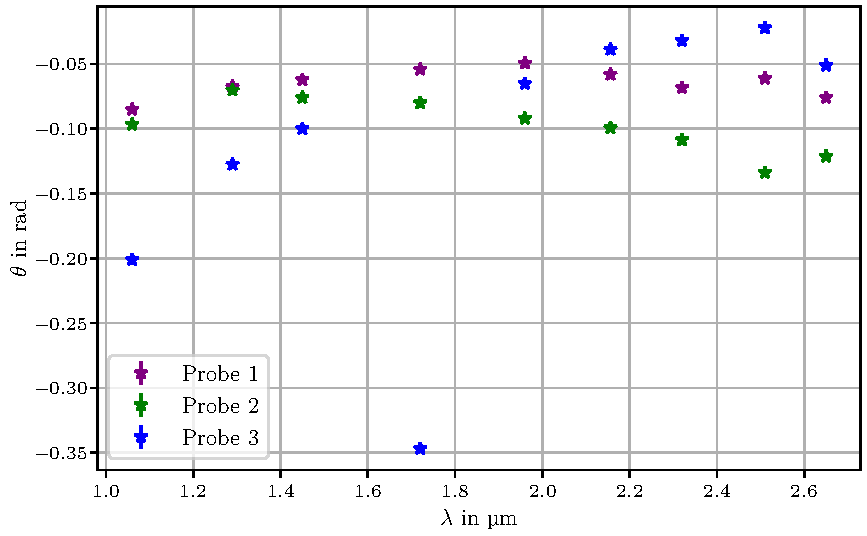
\includegraphics[width=\textwidth]{plots/raw_data.pdf}
    \caption{$\theta$ in Abhängigkeit von der Wellenlänge $\lambda$.}
    \label{fig:rawdata}
\end{figure}

=======
\begin{table}[H]
    \centering
    \caption{Gemessene Polarisationswinkel für Probe 3 mit $N = \qty{0}{\per\cubic\centi\meter}$ und Dicke $d = \qty{5.11}{\milli\meter}$.}
    \label{tab:probe3}
    \begin{tabular}{c c c c}
        \toprule
        {$\lambda$ in $\si{\micro\meter}$} & {$\theta_1$ in $\si{\degree}$} & {$\theta_2$ in $\si{\degree}$} & {$\theta_\text{frei}$ in $\si{\radian}$} \\
        \midrule
        1,06  & 66,28 & 89,33 & $\num{39.36(1)}$ \\
        1,29  & 70,40 & 85,00 & $\num{24.93(1)}$ \\
        1,45  & 73,25 & 84,70 & $\num{19.55(1)}$ \\
        1,72  & 41,00 & 80,76 & $\num{67.90(1)}$ \\
        1,96  & 68,83 & 76,30 & $\num{12.75(1)}$ \\
        2,156 & 65,91 & 70,35 & $\num{7.58(1)}$  \\
        2,34  & 42,71 & 46,38 & $\num{6.26(1)}$ \\
        2,51  & 29,71 & 32,25 & $\num{4.33(1)}$ \\
        2,65  & 59,33 & 65,18 & $\num{9.99(1)}$ \\   
        \bottomrule
    \end{tabular}
\end{table}
Zur veranschaulichung der Messergebnisse werden die normierten Winkel in \autoref{fig:rawdata} gegen die Wellenlänge geplottet.
\begin{figure}
    \centering
    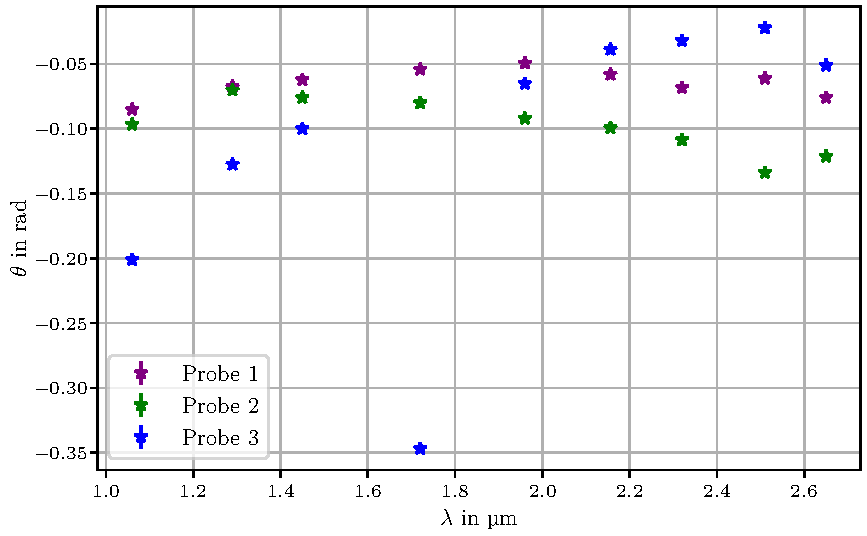
\includegraphics[width=\textwidth]{plots/raw_data.pdf}
    \caption{$\theta$ in Abhängigkeit von der Wellenlänge $\lambda$.}
    \label{fig:rawdata}
\end{figure}

>>>>>>> 488e4e5413ead7ea746f355c1424b3fbb286a0b0

\subsection{Bestimmung der Effektiven Masse}
Um die effektive Masse zu bestimmen, wird gemäß \autoref{eq:theta_frei} eine lineare Regression von $\theta_\text{frei}$ in $\lambda^2$ der Form,
\begin{equation}
<<<<<<< HEAD
f(x)=m \cdot x,
\label{eq:lineareform}
||||||| 05b9994
f(x)=m \cdot x+b,
\label{eq:lineareform}
=======
    f(x)=m \cdot x+b,
    \label{eq:lineareform}
>>>>>>> 488e4e5413ead7ea746f355c1424b3fbb286a0b0
\end{equation}
durchgeführt. Aus der errechneten Steigung $m$ kann die effektive Masse bestimmt werden.\\
Dabei ist zu beachten, dass der Brechungsindex $n$ abhängig von der Wellenlänge ist. Die Regressionen werden einmal mit konstantem $n = \num{3,5}$
und einmal mit variablem $n$ gemäß der Sellmeier-Gleichung,
\begin{equation}
<<<<<<< HEAD
    n(\lambda^2) = \sqrt{\num{8,950} + \frac{\num{2,054}}{1 - \num{0,390} \cdot \lambda^2}}
||||||| 05b9994
    n(\lambda^2) = \sqrt{8.950 + \frac{2.054}{1 - 0.390 \cdot \lambda^2}}
=======
    n(\lambda^2) = \sqrt{\qty{8.950} + \frac{\qty{2.054}}{1 - \qty{0.390} \cdot \lambda^2}}
>>>>>>> 488e4e5413ead7ea746f355c1424b3fbb286a0b0
    \label{eq:sellmeier}
\end{equation}
<<<<<<< HEAD
durchgeführt, wobei $\lambda$ in $\si{\micro\meter}$ sein muss \cite{sellmeier}.
||||||| 05b9994
durchgeführt, wobei $\lambda$ in $\si{\micro\meter}$ sein muss.
=======
durchgeführt, wobei $\lambda$ in der Größenordnung $\si{\micro\meter}$ gegeben sein muss.
>>>>>>> 488e4e5413ead7ea746f355c1424b3fbb286a0b0

\subsubsection{Konstanter Brechungsindex}
Die effektive Masse berechnet sich nach \autoref{eq:theta_frei} mit konstantem $n = \num{3,5}$ über
\begin{equation}
    m^* = \sqrt{\frac{e_0^3 N B}{8 \pi^2 \epsilon c^3} \cdot \frac{1}{mn}}.
\label{eq:masse}
\end{equation}
Dabei ist $e_0 = \qty{1.603e-19}{\coulomb}$ die Elementarladung, $\epsilon = \num{12.4} \cdot \epsilon_0 = \num{12.4} \cdot \qty{8.85e-12}{\farad\per\meter} = \qty{1.0974e-10}{\farad\per\meter}$ die Dielektrizitätskonstante des Materials,
$c= \qty{3e8}{\meter\per\second}$ die Lichtgeschwindigkeitund $B= \qty{412.0}{\milli\tesla}$ die maximale Kraftflussdichte. $N$ ist die Dotierungskonzentration. $m$ ist die Steigung der linearen Fits.\\
In \autoref{fig:regression1} ist $\theta_\text{frei, dot} - \theta_\text{frei, undot}$ gegen $\lambda^2$ mit dem entstandenen Fit dargestellt.
\begin{figure}
    \centering
    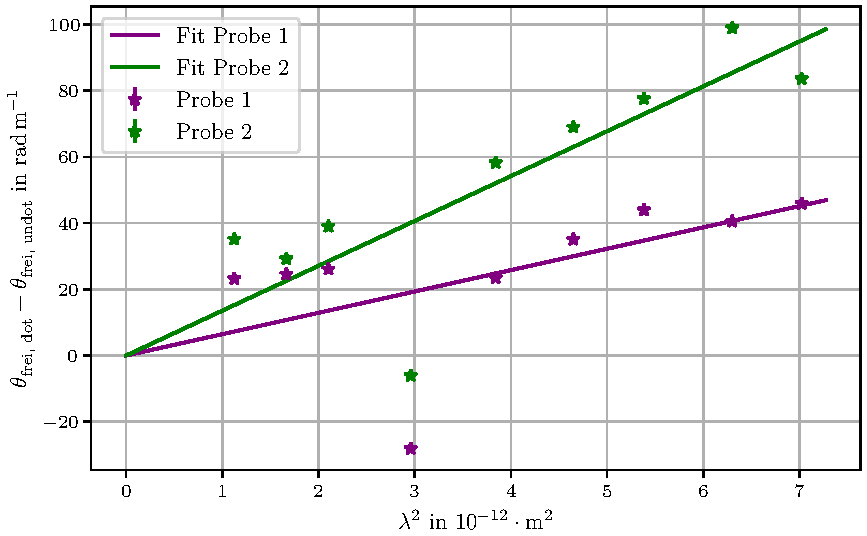
\includegraphics[width=\textwidth]{plots/fits_ohne_n.pdf}
    \caption{Lineare Regression über $\theta_\text{frei}$ gegen $\lambda^2$ mit konstantem $n$.}
    \label{fig:regression1}
\end{figure}
Die Fitparameter für \autoref{fig:regression1} lauten
<<<<<<< HEAD
||||||| 05b9994
\begin{align*}
    m &= \qty{0.0296(156)}{\radian\per\square\micro\meter} \\
    b &= \qty{-0.1600(679)}{\radian}.
\end{align*}
für $N = \qty{1.2e18}{\cubic\centi\meter}$, was einer effektiven Masse von
=======
\begin{align*}
    m &= \qty{5.3(3.4)}{\radian\per\square\micro\meter} \\
    b &= \qty{4.7+-15.0}{\radian}.
\end{align*}
für $N = \qty{1.2e18}{\cubic\centi\meter}$, was einer effektiven Masse von
>>>>>>> 488e4e5413ead7ea746f355c1424b3fbb286a0b0
\begin{equation*}
<<<<<<< HEAD
    m_{1, \text{n konst.}} = \qty{6.4519(35)e18}{\radian\per\meter\cubed} 
\end{equation*}
für $N = \qty{1.2e18}{\cubic\centi\meter}$, was einer effektiven Masse von 
\begin{equation*}
    m^*_{1, \text{n konst.}} = \qty{1.9848(6)e-32}{\kilo\gram}
||||||| 05b9994
    m^* = \qty{2.9(8)e-31}{\kilo\gram}
=======
    m^* = \qty{2.2(7)e-32}{\kilo\gram}
>>>>>>> 488e4e5413ead7ea746f355c1424b3fbb286a0b0
\end{equation*}
entspricht, und
<<<<<<< HEAD
||||||| 05b9994
\begin{align*}
    m &= \qty{0.0386(156)}{\radian\per\square\micro\meter} \\
    b &= \qty{-0.1623(682)}{\radian}.
\end{align*}
für $N = \qty{2.8e18}{\cubic\centi\meter}$, was einer effektiven Masse von
=======
\begin{align*}
    m &= \qty{12.4(3.5)}{\radian\per\square\micro\meter} \\
    b &= \qty{5.3+-15.3}{\radian}.
\end{align*}
für $N = \qty{2.8e18}{\cubic\centi\meter}$, was einer effektiven Masse von
>>>>>>> 488e4e5413ead7ea746f355c1424b3fbb286a0b0
\begin{equation*}
<<<<<<< HEAD
    m_{2, \text{n konst.}} = \qty{13.5534(37)e18}{\radian\per\meter\cubed} 
\end{equation*}
für $N = \qty{1.2e18}{\cubic\centi\meter}$, was einer effektiven Masse von 
\begin{equation*}
    m^*_{2, \text{n konst.}} = \qty{2.0917(3)e-32}{\kilo\gram}
\end{equation*}
||||||| 05b9994
    m^* = \qty{3.9(8)e-31}{\kilo\gram}
\end{equation*} 
=======
    m^* = \qty{2.18(31)e-32}{\kilo\gram}
\end{equation*} 
>>>>>>> 488e4e5413ead7ea746f355c1424b3fbb286a0b0
entspricht.


\subsubsection{Variabler Brechungsindex}
Gemäß der Sellmeier-Gleichung \ref{eq:sellmeier} finden sich die Brechungsindizes zu
\begin{table}[H]
    \centering
    \caption{Brechungsindizes $n$ zu den Wellenlängen $\lambda$ in $\si{\micro\meter}$ nach \autoref{eq:sellmeier}.}
    \label{tab:sellmeyer}
    \begin{tabular}{c c c c c c c c c c}
        \toprule
        {$\lambda$} & 1,06 & 1,29 & 1,45 & 1,72 & 1,96 & 2,156 & 2,32 & 2,51 & 2,65 \\
        \midrule
        {$n$} & 3,478 & 3,410 & 3,387 & 3,364 & 3,352 & 3,345 & 3,341 & 3,338 & 3,335 \\
        \bottomrule
    \end{tabular}
\end{table}
Die effektive Masse berechnet sich nach \autoref{eq:theta_frei} über
\begin{equation}
    m^* = \sqrt{\frac{e_0^3 N B}{8 \text{\pi}^2 \epsilon c^3} \cdot \frac{1}{m}}.
\label{eq:masse}
\end{equation}
Die Brechungsindizes $n$ aus \autoref{tab:sellmeyer} sind nun nicht mehr in der Gleichung, da diese in $m$ berücksichtigt sind.\\
In \autoref{fig:regression2} ist $\theta_\text{frei, dot} - \theta_\text{frei, undot}$ gegen $\frac{\lambda^2}{n}$ mit dem entstandenen Fit dargestellt.
\begin{figure}
    \centering
    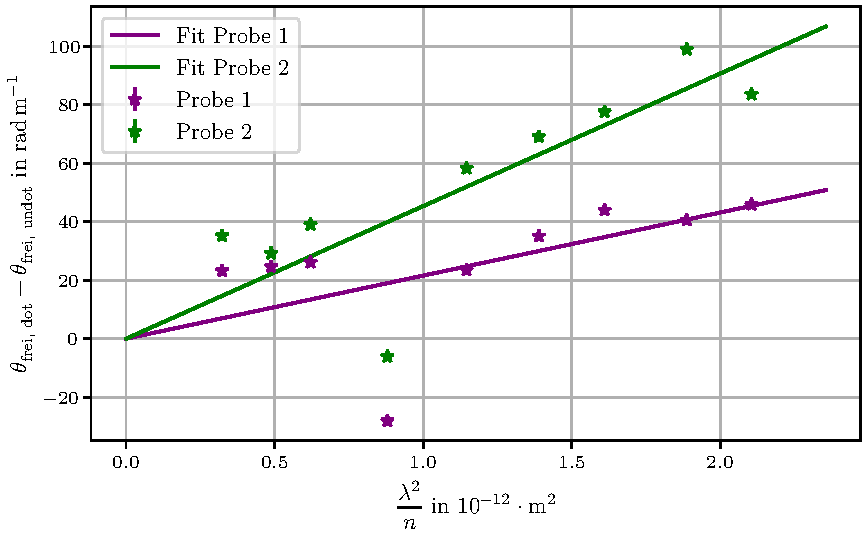
\includegraphics[width=\textwidth]{plots/fits_mit_n.pdf}
    \caption{Lineare Regression über $\theta_\text{frei}$ gegen $\frac{\lambda^2}{n}$ mit variablen $n$.}
    \label{fig:regression2}
\end{figure}

Die Fitparameter für \autoref{fig:regression2} lauten
<<<<<<< HEAD
||||||| 05b9994
\begin{align*}
    m &= \qty{0.10(5)}{\radian\per\square\micro\meter} \\
    b &= \qty{-0.16(7)}{\radian}.
\end{align*}
für $N = \qty{1.2e18}{\cubic\centi\meter}$, was einer effektiven Masse von
=======
\begin{align*}
    m &= \qty{18(11)}{\radian\per\square\micro\meter} \\
    b &= \qty{5(15)}{\radian}.
\end{align*}
für $N = \qty{1.2e18}{\cubic\centi\meter}$, was einer effektiven Masse von
>>>>>>> 488e4e5413ead7ea746f355c1424b3fbb286a0b0
\begin{equation*}
<<<<<<< HEAD
    m_{1, \text{n var.}} = \qty{21.567(12)e18}{\radian\per\meter\cubed} 
\end{equation*}
für $N = \qty{1.2e18}{\cubic\centi\meter}$, was einer effektiven Masse von 
\begin{equation*}
    m^*_{1, \text{n var.}} = \qty{1.0855(3)e-32}{\kilo\gram}
||||||| 05b9994
    m^* = \qty{1.6(4)e-31}{\kilo\gram}
=======
    m^* = \qty{1.20(40)e-32}{\kilo\gram}
>>>>>>> 488e4e5413ead7ea746f355c1424b3fbb286a0b0
\end{equation*}
entspricht, und
<<<<<<< HEAD
||||||| 05b9994
\begin{align*}
    m &= \qty{0.13(5)}{\radian\per\square\micro\meter} \\
    b &= \qty{-0.16(7)}{\radian}.
\end{align*}
für $N = \qty{2.8e18}{\cubic\centi\meter}$, was einer effektiven Masse von
=======
\begin{align*}
    m &= \qty{41(12)}{\radian\per\square\micro\meter} \\
    b &= \qty{6(15)}{\radian}.
\end{align*}
für $N = \qty{2.8e18}{\cubic\centi\meter}$, was einer effektiven Masse von
>>>>>>> 488e4e5413ead7ea746f355c1424b3fbb286a0b0
\begin{equation*}
<<<<<<< HEAD
    m_{2, \text{n var.}} = \qty{45.316(13)e18}{\radian\per\meter\cubed} 
\end{equation*}
für $N = \qty{1.2e18}{\cubic\centi\meter}$, was einer effektiven Masse von 
\begin{equation*}
    m^*_{2, \text{n var.}} = \qty{1.1439(2)e-32}{\kilo\gram}
\end{equation*}
||||||| 05b9994
    m^* = \qty{2.2(4)e-31}{\kilo\gram}
\end{equation*} 
=======
    m^* = \qty{1.20(17)e-32}{\kilo\gram}
\end{equation*} 
>>>>>>> 488e4e5413ead7ea746f355c1424b3fbb286a0b0
entspricht.